\documentclass[MAS331_Note.tex]{subfiles}

\begin{document}

\chapter{Countability and Separation Axioms}

\section{The Countability Axioms}

\dfn{First Countability Axiom}{
    A topological space $X$ is said to have a \textit{countable basis at} $x$
    if there is a countable collection $\mcal B$ of neighborhoods of $x$ in $X$
    such that, for each neighborhood $U$ of $x$, there exists $B \in \mcal B$
    with $B \subseteq U$. A space that has a countable basis at each point is
    said to satisfy the \textit{first countability axiom}, or to be
    \textit{first-countable}.
}

\nt{
    This definition was already given in \Cref{def:1stCt}.
    Recall the lemmas \Cref{lem:seqLemma} and \Cref{lem:seqConvIffImgConv}.
}

\dfn{Second Countability Axiom}{
    If a topological space $X$ has a countable basis for its topology, then
    $X$ is said to satisfy the \textit{second countability axiom}, or to be
    \textit{second-countable}.
}

\exmp{}{
    $\RR[J]$ endowed with the product topology with a countable set $J$ is
    second-countable;
    \[
        \mcal S \triangleq \bigcup_{\alpha \in J} \big\{\, \pi_{\alpha}\inv
        \big((a, b)\big) \:\big|\: a, b \in \QQ \text{ and } a<b \big\}
    \]
    is a countable subbasis for $\RR[J]$, which induces a countable basis for
    $\RR[J]$.
}

\nt{
    If a topological space $X$ is second-countable with a countable basis
    $\mcal B= \{B_n\}_{n \in \ZZ_+}$ and a subspace $A \subseteq X$ with the
    discrete topology. Then, $A$ must be countable.

    Otherwise, for each $a \in A$, there exists $B_a \in \mcal B$ such that
    $B_a \cap A = \{a\}$. This induces an injection $A \hookrightarrow \mcal B$.
    Hence, $A$ is countable.
}

\exmp[RUnifNot2ndCt]{Uniform Topology and Countability Axioms}{
    In the uniform topology, $\RR[\omega]$ is first-countable by
    \Cref{exmp:metIs1stCt}. Let $\mcal B$ be a basis of $\RR[\omega]$. Let
    \[
        A \triangleq \big\{\,(x_i)_{i \in \ZZ_+} \in \RR[\omega] \:\big|\:
        \fall i \in \ZZ_+,\: x_i \in \{\,0, 1\,\}\,\big\}\text{.}
    \]
    Then, $A$ has the discrete topology but $A$ is uncountable. Therefore,
    $\RR[\omega]$ with the uniform topology is not second-countable.
}

\thm[subspCt]{}{
    Let $X$ be a topological space and $A$ be a subspace of $X$.
    \begin{itemize}[nolistsep]
        \ii If $X$ is first-countable, then $A$ is first-countable.
        \ii If $X$ is second-countable, then $A$ is second-countable.
    \end{itemize}
}
\pf{Proof}{
    \hfill
    \begin{itemize}[nolistsep]
        \ii Let $a \in A$. Let $\mcal B$ be a countable basis of $X$ at $a$.
            Then, $\{\,B \cap A \mid B \in \mcal B\,\}$ is a countable basis
            for the subspace $A$ at $a$. \checkmark
        \ii Let $\mcal B$ be a countable basis of $X$. Then, $\{\,B \cap A
            \mid B \in \mcal B\,\}$ is a countable basis for the subspace $A$.
            \checkmark
    \end{itemize}
}

\thm[prodCt]{}{
    Let $\{X_\alpha\}_{\alpha \in J}$ be a countable family of topological
    spaces.
    \begin{itemize}[nolistsep]
        \ii If each $X_i$ is first-countable, then $\prod_{\alpha \in J}
            X_\alpha$ in the product topology is first-countable.
        \ii If each $X_i$ is second-countable, then $\prod_{\alpha \in J}
            X_\alpha$ in the product topology is second-countable.
    \end{itemize}
}
\pf{Proof}{
    \hfill
    \begin{itemize}[nolistsep]
        \ii Let $(x_{\alpha})_{\alpha \in J} \in \prod_{\alpha \in J} X_\alpha$.
            Then, for each $\alpha \in J$, there exists a countable basis
            $\mcal B_\alpha$ of $X_\alpha$ at $x_\alpha$.
            Then, $\big\{\, \prod_{\alpha \in J} B_\alpha \:\big|\:
            \fall \alpha \in J,\: B_\alpha \in \mcal B_\alpha\,\big\}$ is a
            countable basis at $(x_\alpha)_{\alpha \in J}$.
        \ii For each $\alpha \in J$, there exists a countable basis $\mcal
            B_\alpha$ of $X_\alpha$. Then, $\big\{\,\prod_{\alpha \in J}
            B_\alpha \:\big|\: \fall \alpha \in J,\: B_\alpha \in \mcal
            B_\alpha\,\big\}$ is a countable basis of $\prod_{\alpha \in J}
            X_\alpha$.
    \end{itemize}
}

\dfn{Lindelöf Space}{
    A topological space $X$ is called a \textit{Lindelöf space} if, for every
    open covering of $X$, there is a countable subcovering.
}

\dfn{Dense Subset}{
    A subset $A$ of a topological space $X$ is said to be \textit{dense} in $X$
    if $\cl A = X$.
}

\dfn{Separable Space}{
    A topological space $X$ is said to be \textit{separable} if there is a
    countable dense subset of $X$.
}

\nt{
    Obvious facts:
    \begin{itemize}[nolistsep]
        \ii Every compact space is a Lindelöf space.
        \ii The box and product topologies on an finite product of separable
            spaces is separable.
            (\Cref{th:prodOfClosureIsClosureOfProd})
        \ii Every topology on a countable set is Lindelöf and separable.
   \end{itemize}
}

\thm[2ndCtThenLindAndSep]{}{
    Let $X$ be a second-countable space. Then,
    \begin{itemize}[nolistsep]
        \ii $X$ is a Lindelöf space.
        \ii $X$ is separable.
    \end{itemize}
}
\pf{Proof}{
    Let $\mcal B = \{B_n\}_{n \in \ZZ_+}$ be a countable basis for $X$.
    \begin{itemize}[nolistsep]
        \ii Let $\mcal A$ be an open covering of $X$. For each $n \in \ZZ_+$,
            there exists $A_n \in \mcal A$ such that $B_n \subseteq A_n$.
            Then, $\mcal A' \triangleq \{\,A_n \mid n \in \ZZ_+\,\}$ is a
            countable subcovering of $X$ as $\mcal B$ covers $X$. \checkmark
        \ii For each $n \in \ZZ_+$, choose $x_n \in B_n$. Let $D \triangleq
            \{\,x_n \mid n \in \ZZ_+\,\}$. Then, for all $x \in X$, every
            basis element that contains $x$ intersects $D$; $\cl D = X$
            by \Cref{th:inClosureIffNeighCapANonempty}. \checkmark
    \end{itemize}
}

\exmp[REllCt]{$\RR_\ell$ and Countability Axioms}{
    \begin{itemize}[nolistsep]
        \ii Given $x \in \RR_\ell$, $\{\,[x, x + 1/n) \mid n \in \ZZ_+\,\}$
            is a countable basis at $x$. $\RR_\ell$ is first-countable.
        \ii $\cl{\QQ} = \RR_\ell$. $\RR_\ell$ is separable.
        \ii Let $\mcal B$ be a basis for $\RR_\ell$. Choose, for each $x \in
            \RR_\ell$, an element $B_x \in \mcal B$ such that $x \in B_x
            \subseteq [x, x+1)$. If $x \neq y$, then $B_x \neq B_y$. Hence
            $x \mapsto B_x$ is an injection; $\mcal B$ is uncountable.
            Therefore, $\RR_\ell$ is not second-countable.
    \end{itemize}
    We now prove $\RR_\ell$ is Lindelöf. Thanks to \Cref{lem:topByBIsUnionsOfB},
    we only have to prove that, for any open covering $\mcal A$ of $\RR_\ell$
    by the basis elements, there is a countable subcovering.

    Let $\mcal A = \{\,[a_\alpha, b_\alpha) \mid \alpha \in J\,\}$ be an open
    covering of $\RR_\ell$. Let $C \triangleq \bigcup_{\alpha \in J} (a_\alpha,
    b_\alpha)$. We now claim that $\RR \setminus C$ is countable.
    Let $x \in \RR \setminus C$. Then $x = a_\beta$ for some $\beta \in J$.
    Choose $q_x \in \QQ$ such that $q_x \in (a_\beta, b_\beta)$.
    If $x, y \in \RR \setminus C$ and $x < y$, then $q_x < q_y$. Hence
    $x \mapsto q_x$ defines an injection $\RR \setminus C \hookrightarrow \QQ$.
    Therefore, $\RR \setminus C$ is countable.

    Now, let $\mcal A'$ be a countable subcollection of $\mcal A$ that covers
    $\RR \setminus C$. Now, note that $\{\,(a_\alpha, b_\alpha) \mid \alpha \in
    J\,\}$ is an open covering of $C$ as a subspace of $\RR$ (with the standard
    topology). Since $\RR$ is second-countable, there exists a finite
    subcollection $\{\,(a_{\alpha_1}, b_{\alpha_1}), \cdots, (a_{\alpha_n},
    b_{\alpha_n})\,\}$ covers $C$. Let $\mcal A'' \triangleq \{\,[a_{\alpha_1},
    b_{\alpha_1}), \cdots, [a_{\alpha_n}, b_{\alpha_n})\}$.
    Then, $\mcal A' \cup \mcal A''$ is a countble subcovering of $\RR_\ell$.
}

\exmp[sorgenfrey]{The Product of Two Lindelöf Spaces Need Not Be Lindelöf}{
    Although $\RR_\ell$ is Lindelöf, $\RR_\ell \times \RR_\ell$ is not.
    Consider the subspace $L \triangleq \{\,x \times (-x) \mid x \in
    \RR_\ell\}$. Then, $L$ has the discrete topology as $\big([x, x+1) \times
    [-x, -x+1)\big) \cap L = \{x \times (-x)\}$. Hence, $L$ is not Lindelöf;
    $\RR_\ell^2$ is not Lindelöf.
}

\exmp{A Subspace of a Lindelöf Space Need Not Be Lindelöf}{
    The ordered square $I_o^2$ is compact (\Cref{exmp:orderedSqIsCpt}) and thus
    is Lindelöf. However, the subspace $A = I \times (0, 1)$ is not Lindelöf
    as an open covering $\{\,\{x\} \times (0, 1) \mid x \in I\,\}$ does not
    allow a countable subcovering.
}

\nt{
    Here is the diagram that represents the relations between spaces.
    \begin{center}
    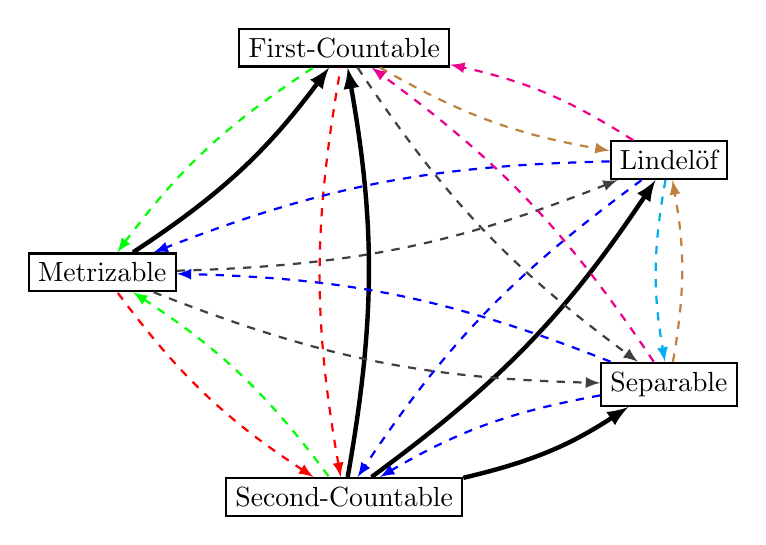
\begin{tikzpicture}[thick]
        \node[draw] (met) at (180:4) {Metrizable};
        \node[draw] (first) at (108:3) {First-Countable};
        \node[draw] (second) at (-108:3) {Second-Countable};
        \node[draw] (lind) at (24:3.5) {Lindelöf};
        \node[draw] (sep) at (-24:3.5) {Separable};

        \draw[->, >=latex, bend right=10, ultra thick] (met) edge (first);
        \draw[<-, >=latex, bend left=10, green] (met) edge[dashed] (first);
        \draw[->, >=latex, bend right=10, ultra thick] (second) edge (first);
        \draw[<-, >=latex, bend left=10, red] (second) edge[dashed] (first);
        \draw[<-, >=latex, bend left=10, green] (met) edge[dashed] (second);
        \draw[<-, >=latex, bend left=10, red] (second) edge[dashed] (met);
        \draw[->, >=latex, bend right=10, ultra thick] (second) edge (lind);
        \draw[->, >=latex, bend right=10, ultra thick] (second) edge (sep);
        \draw[->, >=latex, bend right=10, blue] (lind) edge[dashed] (met);
        \draw[->, >=latex, bend right=10, blue] (sep) edge[dashed] (met);
        \draw[->, >=latex, bend right=10, blue] (lind) edge[dashed] (second);
        \draw[->, >=latex, bend right=10, blue] (sep) edge[dashed] (second);
        \draw[->, >=latex, bend right=10, brown] (sep) edge[dashed] (lind);
        \draw[->, >=latex, bend right=10, brown] (first) edge[dashed] (lind);
        \draw[->, >=latex, bend right=10, darkgray] (met) edge[dashed] (lind);
        \draw[->, >=latex, bend right=10, darkgray] (met) edge[dashed] (sep);
        \draw[->, >=latex, bend right=10, darkgray] (first) edge[dashed] (sep);
        \draw[->, >=latex, bend right=10, magenta] (sep) edge[dashed] (first);
        \draw[->, >=latex, bend right=10, magenta] (lind) edge[dashed] (first);
        \draw[->, >=latex, bend right=10, cyan] (lind) edge[dashed] (sep);
    \end{tikzpicture}
    \end{center}
    Counterexamples:
    \begin{itemize}[nolistsep]
        \ii ({\color{green}$\dashrightarrow$}) $X = \{0, 1\}$ with $\mcal T =
            \{\OO, X, \{0\}\}$ is second-countable but not Hausdorff,
            thus not metrizable.
        \ii ({\color{red}$\dashrightarrow$})
            $\RR[\omega]$ with the uniform topology is metrizable but not
            second-countable. (\Cref{exmp:RUnifNot2ndCt})
        \ii ({\color{blue}$\dashrightarrow$})
            $\RR_\ell$ ($\RR$ with the lower limit topology) is
            first-countable, Lindelöf, and separable; but it is neither
            second-countable nor metrizable. (\Cref{exmp:REllCt})
        \ii ({\color{brown}$\dashrightarrow$})
            $\RR_\ell \times \RR_\ell$ is first countable and separable, but
            it is not Lindelöf. (\Cref{exmp:sorgenfrey})
        \ii ({\color{darkgray}$\dashrightarrow$})
            $\RR$ with the discrete topology is first-countable and metrizable;
            but it is not second-countable, separable, or Lindelöf.
        \ii ({\color{magenta}$\dashrightarrow$})
            $\RR$ with the finite complement topology is separable and
            Lindelöf; but it is neither first-countable nor metrizable.
        \ii ({\color{cyan}$\dashrightarrow$})
            $\RR$ with the countable complement topology is Lindelöf;
            but it is not first-countable, metrizable, or separable.
    \end{itemize}
}

\section{Separation Axioms}

\dfn{Regular and Normal Space}{
    Let $X$ be a topological space that $\{x\}$ is closed for every $x \in X$.
    In other words, $X$ is $T_1$.
    \begin{itemize}[nolistsep]
        \ii $X$ is said to be $T_2$ if it is Hausdorff.
        \ii $X$ is said to be \textit{regular}, or $T_3$, if, for each $x \in X$
            and a closed set $B$ disjoint from $x$, there exist disjoint open
            sets $U$ and $V$ such that $x \in U$ and $B \subseteq V$.
        \ii $X$ is said to be \textit{normal}, or $T_4$, if, for each pair $A$,
            $B$ of disjoint closed sets in $X$, there exist disjoint open sets
            $U$ and $V$ such that $A \subseteq U$ and $B \subseteq V$.
    \end{itemize}
}

\nt{
    \[
        T_1 \supseteq T_2 \supseteq T_3 \supseteq T_4
    \]
}

\exmp[RKisT2butNotT3]{$T_2$ Does Not Imply $T_3$}{
    The space $\RR_K$ is $T_2$ as it is finer than the standard topology.
    The set $K = \{\,1/n \mid n \in \ZZ_+\,\}$ is closed in $\RR_K$ and
    $0 \notin K$. Suppose there are disjoint open sets $U$ and $V$ such that
    $0 \in U$ and $K \subseteq V$. Let $B$ be a basis element that $0 \in B
    \subseteq U$. Then, $B = (a, b) \setminus K$ since any open interval
    containing $0$ intersects $K$. (It must be $a < 0 < b$.) Let $n \in \ZZ_+$
    such that $1/n < b$. Then, $1/n \in K \subseteq V$. Let $B'$ be a basis
    element such that $1/n \in B' \subseteq V$. Then, $B' = (c, d)$ for some
    $c < d$. Let $\max \{\,c, 1/(n+1)\,\} < z < 1/n$. Then, $z \in B \cap B'
    \subseteq U \cap V$. Hence, $\RR_K$ is not $T_3$, \#.
}

\mlemma[T34Iff]{Another Formulation}{
    Let $X$ be a $T_1$ space.
    \begin{enumerate}[nolistsep, label=(\roman*)]
        \ii $X$ is $T_3$ if and only if, for each $x \in U$ and a neighborhood
            $U$ of $x$, there exists a neighborhood $V$ of $x$ such that
            $\cl V \subseteq U$.
        \ii $X$ is $T_4$ if and only if, for each closed set $A$ and an open
            set $U$ containing $A$, there exists an open set $V$ such that
            $A \subseteq V$ and $\cl V \subseteq U$.
    \end{enumerate}
}
\pf{Proof}{
    \hfill
    \begin{enumerate}[nolistsep, label=(\roman*)]
        \ii ($\Rightarrow$)
            $B \triangleq X \setminus U$ is a closed set and $x \notin B$; there
            exist disjoint open sets $V$ and $W$ such that $x \in V$ and
            $B \subseteq W$. Then, $\cl V$ does not intersect $B$, i.e.,
            $\cl V \subseteq U$. \checkmark

            ($\Leftarrow$)
            Let $x \in X$ and $B \subseteq X$ be a closed set with $x \notin B$.
            Then, $X \setminus B$ is a neighborhood of $x$; there exists a
            neighborhood $V$ of $x$ such that $\cl V \subseteq X \setminus B$.
            Then, $V$ and $X \setminus \cl V$ are disjoint open sets that
            contain $x$ and $B$, respectively. \checkmark

        \ii ($\Rightarrow$)
            $B \triangleq X \setminus U$ is a closed set and $A \cap B =
            \OO$; there exist disjoint open sets $V$ and $W$ such that
            $A \subseteq V$ and $B \subseteq W$. Then, $\cl V$ does not
            intersect $B$, i.e., $\cl V \subseteq U$. \checkmark

            ($\Leftarrow$)
            Let $A, B \subseteq X$ be disjoint closed sets in $X$. Then,
            $X \setminus B$ is an open set that contains $A$; there exists an
            open set $V$ such that $A \subseteq V$ and $\cl V \subseteq X
            \setminus B$. Then, $V$ and $X \setminus \cl V$ are disjoint open
            sets that contain $A$ and $B$, respectively. \checkmark
    \end{enumerate}
}

\thm[subspSep]{}{
    Let $X$ be a topological space and $Y \subseteq X$ be a subspace of $X$.
    \begin{enumerate}[nolistsep, label=(\roman*)]
        \ii If $X$ is $T_1$, then $Y$ is $T_1$.
        \ii If $X$ is $T_2$, then $Y$ is $T_2$.
        \ii If $X$ is $T_3$, then $Y$ is $T_3$.
    \end{enumerate}
}
\pf{Proof}{
    \hfill
    \begin{enumerate}[nolistsep, label=(\roman*)]
        \ii For each $x \in Y$, $\{x\} \cap Y = \{x\}$ is closed.
        \ii Let $x, y \in Y$ with $x \neq y$.
            Then, there exist disjoint neighborhoods $U$ and $V$ of $x$ and $y$,
            respectively, in $X$. Then, $U \cap Y$ and $V \cap Y$ are disjoint
            neighborhoods of $x$ and $y$ in $Y$, respectively.
        \ii $Y$ is already $T_1$ by (i). Let $x \in Y$ and $B$ be a closed
            set in $Y$ disjoint from $x$. Then, $\cl B \cap Y = B$ by
            \Cref{th:closureSubspace}. Hence, $x \notin \cl B$; there are
            disjoint open sets $U$ and $V$ in $X$ such that $x \in U$ and $\cl
            B \subseteq V$. Then, $U \cap Y$ and $V \cap Y$ are disjoint open
            sets and $x \in U \cap Y$ and $B \subseteq V \cap Y$.
    \end{enumerate}
}

\thm[prodSep]{}{
    Let $\{X_\alpha\}_{\alpha \in J}$ be a family of topological spaces.
    Let $X \triangleq \prod_{\alpha \in J} X_\alpha$ be endowed with either
    box or product toplogy.
    \begin{enumerate}[nolistsep, label=(\roman*)]
        \ii $X$ is $T_1$ if and only if each $X_\alpha$ is $T_1$.
        \ii $X$ is $T_2$ if and only if each $X_\alpha$ is $T_2$.
        \ii $X$ is $T_3$ if and only if each $X_\alpha$ is $T_3$.
    \end{enumerate}
}
\pf{Proof}{
    Let $\vec x = (x_\alpha)_{\alpha \in J} \in X$.
    Supopse $X$ is $T_1$(, $T_2$, or $T_3$). Then, For each $\alpha_0 \in J$,
    $X_{\alpha_0}$ is homeomorphic with the subspace
    \[
        Y \triangleq \{\,\vec y \in X \mid \fall \alpha \in J \setminus \{
        \alpha_0\},\: y_\alpha = x_\alpha\,\}\text{.}
    \]
    Hence, $X_{\alpha_0}$ is $T_1$(, $T_2$, or $T_3$).
    \begin{enumerate}[nolistsep, label=(\roman*)]
        \ii ($\Leftarrow$)
            Let $\vec x = (x_\alpha)_{\alpha \in J} \in X$.
            Then, $\{\vec x\} = \bigcap_{\alpha \in J} \pi_\alpha\inv
            (\{x_\alpha\})$ is closed.

        \ii ($\Leftarrow$)
            Let $\vec x, \vec y \in X$ with $\vec x \neq \vec y$. Then, there
            exists $\alpha_0 \in J$ such that $x_{\alpha_0} \neq y_{\alpha_0}$;
            there are disjoint neighborhoods $U_{\alpha_0}$ and $V_{\alpha_0}$
            of $x_{\alpha_0}$ and $y_{\alpha_0}$ in $X_{\alpha_0}$. Then,
            If we define $U, V \subseteq X$ by $U \triangleq \prod_{\alpha \in
            J} U_\alpha$ and $V \triangleq \prod_{\alpha \in J} V_\alpha$ where
            \[
                U_\alpha \triangleq \begin{cases}
                    U_{\alpha_0} & \text{if } \alpha = \alpha_0 \\
                    X_\alpha     & \text{otherwise}
                \end{cases} \quad\text{and}\quad
                V_\alpha \triangleq \begin{cases}
                    V_{\alpha_0} & \text{if } \alpha = \alpha_0 \\
                    X_\alpha     & \text{otherwise,}
                \end{cases}
            \]
            we find that $U$ and $V$ are disjoint neighborhoods of $\vec x$ and
            $\vec y$ in $X$.

        \ii ($\Leftarrow$)
            Let $\vec x \in X$ and let $U$ be a neighborhood of $\vec x$ in $X$.
            Choose a basis element $B = \prod_{\alpha \in J} U_\alpha$ so that
            $\vec x \in B \subseteq U$. For each $\alpha \in J$, let $V_\alpha
            = X_\alpha$ if $U_\alpha = X_\alpha$. Otherwise, by
            \Cref{lem:T34Iff}, let $V_\alpha$ be a neighborhood of $x_\alpha$
            in $X$ such that $\cl{V_\alpha} \subseteq U_\alpha$. Then, $V =
            \prod_{\alpha \in J} V_\alpha$ is a neighborhood of $\vec x$ and
            $\cl V = \prod_{\alpha \in J} \cl{V_\alpha} \subseteq B \subseteq
            U$. By \Cref{lem:T34Iff}, $X$ is $T_3$.
   \end{enumerate}
}

\exmp[RlIsT4]{$\RR_\ell$ Is $T_4$}{
    $\RR_\ell$ is $T_1$ as it is finer than the standard topology. Suppose
    $A$ and $B$ are disjoint closed sets in $\RR_\ell$. For each $a \in A$
    choose a basis element $[a, x_a)$ not intersecting $B$. This is possible
    since $\RR \setminus B$ is open in $\RR_\ell$. Similarly, for each $b \in
    B$, choose a basis element $[b, x_b)$ not intersecting $A$. Then,
    \[
        U \triangleq \bigcup_{a \in A} [a, x_a) \quad\text{and}\quad
        V \triangleq \bigcup_{b \in B} [b, x_b)
    \]
    are disjoint open sets such that $A \subseteq U$ and $B \subseteq V$.
}

\exmp[RlsrIsNotT4]{$\RR_\ell^2$ is not $T_4$}{
    The space $\RR_\ell$ is $T_3$; hence $\RR_\ell^2$ is $T_3$ by
    \Cref{th:prodSep}.

    Suppose $\RR_\ell^2$ is normal for the sake of contradiction. Let $L$ be
    a subspace of $\RR_\ell^2$ where $L \triangleq \{\,x \times (-x) \in \RR^2
    \mid x \in \RR\,\}$. Here are some facts:
    \begin{itemize}[nolistsep]
        \ii $L$ has the discrete topology. Thus, every subset of $L$ is closed
            in $L$, especially.
        \ii $L$ is closed in $\RR_\ell^2$ as it is closed in $\RR^2$, which is
            coarser than $\RR_\ell^2$.
        \ii Every subset $A$ of $L$ is closed in $\RR_\ell^2$.
        \ii For every $\OO \neq A \subsetneq L$, there are disjoint
            open sets $U_A$ and $V_A$ in $\RR_\ell^2$ containing $A$ and $L
            \setminus A$, respectively.
    \end{itemize}
    Here, we define a function $\theta \colon \mcal P(L) \to \mcal P(\QQ^2)$ by
    \[
        A \mapsto \begin{cases}
            \QQ^2 \cap U_A & \text{if } \OO \subsetneq A \subsetneq L \\
            \OO    & \text{if } A = \OO \\
            \QQ^2          & \text{if } A = L\text{.}
        \end{cases}
    \]

    To show $\theta$ is injective, let $\OO \subsetneq A, B \subsetneq
    L$ with $A \neq B$. \textsf{WLOG}, $A \not\subseteq B$; let $x \in A
    \setminus B$. Then, since $x \in L \setminus B$, $x \in U_A \cap V_B$.
    Since $\QQ^2$ is dense in $\RR_\ell^2$ and $U_A \cap V_B$ is open and
    nonempty, there exists $q \in \QQ^2 \cap U_A \cap V_B$. Hence,
    $\QQ^2 \cap U_A \not\subseteq \QQ^2 \cap U_B$. Therefore, $\theta$
    is injective.

    Also, the map $\psi \colon \mcal P(\ZZ_+) \to \RR$ defined by
    \[
        S \mapsto \sum_{i=1}^{\infty} \frac{a_i}{10^i}
    \] is injective where $a_i = 1$ if $i \in S$ and $a_i = 0$ if $i \notin S$.
    Thus, there exists an injective map $\psi' \colon \mcal
    P(\QQ^2) \to L$. Then, $\psi' \circ \theta$ is an injective map from
    $\mcal P(L)$ to $L$, \#. (\Cref{th:noInjSurjWithPSet})

    This shows that
    \begin{enumerate}[nolistsep, label=(\roman*)]
        \ii A product of $T_4$ spaces need not be $T_4$.
        \ii A $T_3$ space need not be $T_4$.
    \end{enumerate}
}

\nt{
    \[
        T_1 \supsetneq T_2 \supsetneq T_3 \supsetneq T_4
    \]
}

\section{Normal Spaces}

\thm[2ndCtT3IsT4]{}{
    Every second-countable $T_3$ space is $T_4$.
}
\pf{Proof}{
    Let $X$ be a regular space with a countable basis $\mcal B$. Let $A$ and
    $B$ be disjoint closed subsets of $X$. For each $x \in
    A$, there exists a neighborhood $U$ of $x$ that does not intersect $B$.
    By \Cref{lem:T34Iff}, there exists a neighborhood $V$ of $x$ such that
    $\cl V \subseteq U$. Finally, choose an element of $\mcal B$ such that
    $x \in B \subseteq V$. Collecting such basis elements, we obtain a
    countable covering of $A$ by open sets whose closures do not intersect $B$.
    Let us denote it by $\{U_n\}_{n \in \ZZ_+}$. Similarly, choose a countable
    collection $\{V_n\}_{n \in \ZZ_+}$ of open sets covering $B$ whose closures
    do not intersect $A$.

    For each $n \in \ZZ_+$ define
    \[
        U_n' \triangleq U_n \setminus \left(\bigcup_{i=1}^n \cl{V_i}\right)
        \quad\text{and}\quad
        V_n' \triangleq V_n \setminus \left(\bigcup_{i=1}^n \cl{U_i}\right)\text{.}
    \]
    Each $U_n'$ and $V_n'$ is open. Moreover, $\{U_n'\}_{n \in \ZZ_+}$ and
    $\{V_n'\}_{n \in \ZZ_+}$ cover $A$ and $B$, respectively, since
    $\cl{V_i}$ and $\cl{U_i}$ does not intersect $A$ and $B$, respectively.

    Let
    \[
        U' \triangleq \bigcup_{n \in \ZZ_+} U_n' \quad\text{and}\quad
        V' \triangleq \bigcup_{n \in \ZZ_+} V_n'\text{.}
    \]
    If there exists $x \in U' \cap V'$, then $x \in U_j' \cap V_k'$ for some
    $j$ and $k$. \textsf{WLOG}, $j \le k$. $x \in U_j' \subseteq U_j$
    but $x \in X \setminus \cl{U_k} \subseteq X \setminus \cl{U_j} \subseteq X
    \setminus  U_j$, \#. Hence, $U'$ and $V'$ are disjoint open sets that
    contain $A$ and $B$, respectively.
}

\thm[metIsT4]{}{
    Every metrizable space is $T_4$.
}
\pf{Proof}{
    Let $X$ be a metrizable space with metric $d$.
    Let $A$ and $B$ be disjoint closed subsets of $X$. For each $a \in A$,
    choose $\veps_a$ so that $B(a, \veps_a) \cap B = \OO$. Similarly,
    for each $b \in B$ choose $\veps_b$ so chat $B(b, \veps_b) \cap A = \OO$.
    Let
    \[
        U \triangleq \bigcup_{a \in A} B(a, \veps_a/2) \quad\text{and}\quad
        V \triangleq \bigcup_{b \in B} B(b, \veps_b/2)\text{.}
    \]
    Then, they are open sets that contain $A$ and $B$, respectively.
    To show they are disjoint, suppose there is $x \in U \cap V$ for the sake
    of contradiction. Then, there are $a \in A$ and $b \in B$ such that
    $x \in B(a, \veps_a/2) \cap B(b, \veps_b/2)$. \textsf{WLOG}, $\veps_a \le \veps_b$.
    From the triangle inequality, we get $d(a, b) < (\veps_a + \veps_b) / 2
    \le \veps_b$; $a \in B(b, \veps_b) \cap A$, which contradicts out construction.
}

\thm[cptHausIsT4]{}{
    Every compact Hausdorff space is $T_4$.
}
\pf{Proof}{
    Let $X$ be a compact Hausdorff space. Let $A$ and $B$ be disjoint closed
    sets in $X$. $A$ and $B$ are compact by \Cref{th:cldInCptIsCpt}. Therefore,
    by \Cref{cor:cptAndPntOutside}, for each $a \in A$, there are disjoint open
    sets $U_a$ and $V_a$ in $X$ such that $a \in U_a$ and $B \subseteq V_a$.
    Since $\{U_a\}_{a \in A}$ covers $A$, $A$ may be covered by finitely many
    sets $U_{a_1}, U_{a_2}, \cdots, U_{a_n}$. Then, let
    \[
        U \triangleq U_{a_1} \cup U_{a_2} \cup \cdots \cup U_{a_n} \quad\text{and}\quad
        V \triangleq V_{a_1} \cap V_{a_2} \cap \cdots \cap V_{a_n}\text{.}
    \]
    They are disjoint open sets containing $A$ and $B$, respectively.
}

\thm[wellOrdIsT4]{}{
    Every well-ordered set $X$ is $T_4$ in the order topology.
}
\pf{Proof}{
    Consider an interval of the form $(x, y]$. If $y$ is the largest element,
    then $(x, y]$ is a basis element. If $y$ is not the largest element, then
    $(x, y] = (x, y')$ where $y'$ is the immediate successor of $y$. Hence,
    $(x, y]$ is always open. \checkmark

    Now let $A$ and $B$ be disjoint closed sets in $X$. First consider the case
    that neither contains the least element. For each $a \in A$, there exists
    a basis element about $a$ disjoint from $B$; it contains some interval
    of the form $(x_a, a]$. Similarly, choose $(y_b, b]$ disjoint from $A$.
    The sets
    \[
        U \triangleq \bigcup_{a \in A} (x_a, a] \quad\text{and}\quad
        V \triangleq \bigcup_{b \in B} (y_b, b]
    \]
    are open sets containing $A$ and $B$, respectively. Suppose $z \in U \cap V$
    for the sake of contradiction. Then $z \in (x_a, a] \cap (y_b, b]$ for some
    $a \in A$ and $b \in B$. \textsf{WLOG}, $a < b$. Then, $a \in (y_b, b]$
    while $(y_b, b] \cap A = \OO$, \#. Hence $U \cap V = \OO$.

    Now consider the case, \textsf{WLOG}, $a_0$, the least element, is
    contained in $A$. Then, since $\{a_0\}$ is both open and closed in $X$,
    we may find $U$ and $V$ for $A \setminus \{a_0\}$ and $B$ like above
    and conclude $U \cup \{a_0\}$ and $V$ are disjoint open sets that
    contain $A$ and $B$, respectively.
}

\nt{
    Actually, \textit{every} order topology is normal.
}

\section{The Urysohn Lemma}

\dfn{Separation by a Continuous Function}{
    If $A$ and $B$ are two subsets of the topological space $X$, and if there
    is a continuous function $f \colon X \to [0, 1]$ such that $f(A) = \{0\}$
    and $f(B) = \{1\}$, we say that $A$ and $B$ \textit{can be separated by
    a continuous function}.
}

\thm[urysohnLem]{Urysohn Lemma}{
    Let $X$ be a normal space. Then, for every disjoint closed subsets $A$ and
    $B$ of $X$, $A$ and $B$ can be separated by a continuous function.
}
\pf{Proof}{
    Let $P \triangleq [0, 1] \cap \QQ$. Let $\{\,p_1, p_2, \cdots\,\} = P$.
    For convenience, let $p_1 = 1$ and $p_2 = 0$. Let $P_n = \{\,p_1, p_2,
    \cdots, p_n\,\}$.
    Inductively define $\{U_p\}_{p \in P}$ as follows.
    \begin{itemize}[nolistsep]
        \ii $U_{p_1} = U_1 \triangleq X \setminus B$.
        \ii Since $A \subseteq U_1$, by \Cref{lem:T34Iff}, there is an open set
            $U_0$ in $X$ such that $A \subseteq U_0$ and $\cl{U_0}
            \subseteq U_1$.
        \ii Suppose $U_p$ is defined for each $p \in P_n$ where $n > 1$, and
            $\fall p, q \in P_n,\: (p < q \implies \cl{U_p} \subseteq U_q)$ (*).        
            then $p_{n+1}$ has  its immediate predecessor $q_1$ and an immediate
            successor $q_2$ in $P_n$. By \Cref{lem:T34Iff}, we may find an open
            set $U_{p+1}$ such that $\cl{U_{q_1}} \subseteq U_{p+1}$ and
            $\cl{U_{p+1}} \subseteq U_{q_2}$. Note that (*) still holds for
            $P_{n+1}$.
    \end{itemize}
    Hence, by mathematcial induction, we may find a collection of open sets
    $\{U_p\}_{p \in P}$ such that
    \[
        \fall p, q \in P,\: \big(p < q \implies \cl{U_p} \subseteq U_q\big)
        \text{.} \qquad(\ast)
    \]
    Now, extend $\{U_p\}_{p \in P}$ to $\{U_p\}_{p \in \QQ}$ by defining
    \[
        \begin{aligned}[t]
            U_p &= \OO &\quad \text{if } p < 0\phantom{.}\\
            U_p &= X   &\quad \text{if } p > 0\text{.}
        \end{aligned}
    \]
    Note that still ($\ast$) holds for $\QQ$.

    Now, define $\QQ(x)$ for each $x \in X$ as following.
    \[
        \QQ(x) \triangleq \{\,p \in \QQ \mid x \in U_p \,\}
    \]
    Note that $\QQ(x) \cap (-\infty, 0) = \OO$ for all $x \in X$ and
    $\QQ \cap (1, \infty) \subseteq \QQ(x)$. Since $\QQ(x)$
    is bounded below and nonempty, we may define $f \colon X \to \RR$ by
    \[
        f(x) \triangleq \inf \QQ(x)
        = \inf\{\,p \in \QQ \mid x \in U_p \,\}\text{.}
    \]
    Note that $\Img f = [0, 1]$ by the argument above.
    Then, the following hold.
    \begin{enumerate}[nolistsep, label=(\roman*)]
        \ii $x \in \cl{U_r} \implies f(x) \le r$.
            \begin{itemize}[nolistsep]
                \ii \textit{Proof}. For every $s > r$, $x \in U_s$. Therefore,
                    $(r, \infty) \cap \QQ \subseteq \QQ(x)$. By definition,
                    we have $f(x) \le r$.
            \end{itemize}
        \ii $x \notin U_r \implies f(x) \ge r$.
            \begin{itemize}[nolistsep]
                \ii \textit{Proof}. For every $s < r$, $x \notin U_s$. Therefore,
                    $(\infty, r) \cap \QQ(x) = \OO$. By definition,
                    we have $f(x) \ge r$.
            \end{itemize}
    \end{enumerate}
    Moreover, if $x \in A$, then $\QQ(x) = [0, \infty) \cap \QQ$; $f(A) = \{0\}$.
    Also, if $x \in B$, then $\QQ(x) = (1, \infty) \cap \QQ$; $f(B) = \{1\}$.

    Now, we prove that $f$ is continuous. Let $(c, d)$ be any open interval
    in $\RR$. To prove $f\inv \big((c, d)\big)$ is open, let $x_0$ be any
    element in the set. We may choose $p, q \in \QQ$ such that
    $c < p < f(x_0) < q < d$ by denseness of $\QQ$ in $\RR$.
    We now assert that $U \triangleq U_q \setminus \cl{U_p}$ is a neighborhood
    of $x$ that is contained in $f\inv \big((c, d)\big)$. If $x \in U$, then
    $f(x) \le q$ by (i) and $f(x) \ge p$ by (2). Hence, $f(U) \subseteq (c, d)$;
    $f$ is continuous.
    Hence, $f' \colon X \to [0, 1]$ obtained by restricting the codomain of $f$
    to $[0, 1]$ is continuous by \Cref{th:constructConti}.
}

\cor{}{
    A topological space $X$ is $T_4$ if and only if every pair $A$, $B$ of
    disjoint closed sets in $X$ can be separated by a continuous function.
}
\pf{Proof}{
    ($\Rightarrow$) \Cref{th:urysohnLem}

    ($\Leftarrow$) If $f$ separates $A$ and $B$, then $f\inv\big([0, 1/2)\big)$
    and $f\inv \big((1/2, 1]\big)$ are disjoint open sets that contain $A$ and
    $B$, respectively.
}

\dfn{Completely Regular Space}{
    A topological space $X$ is \textit{completely regular}, or
    $T_{3 \frac{1}{2}}$, if it is $T_1$ and if each point $x_0$ and each closed
    set $A$ not containing $x_0$, $\{x_0\}$ and $A$ can be separated by a
    continuous function.
}

\thm[subspT3half]{}{
    \begin{enumerate}[nolistsep, label=(\roman*)]
        \ii A subspace of a $T_{3 \frac{1}{2}}$ space is $T_{3 \frac{1}{2}}$.
        \ii Let $\{X_\alpha\}_{\alpha \in J}$ be a family of topological
            spaces. Then, $X = \prod_{\alpha \in J} X_\alpha$ is $T_{3 \frac{1}{2}}$
            if and only if each $X_\alpha$ is $T_{3 \frac{1}{2}}$.
    \end{enumerate}
}
\pf{Proof}{
\begin{enumerate}[nolistsep, label=(\roman*)]
    \ii Let $X$ be $T_{3 \frac{1}{2}}$. Let $Y$ be a subspace of $X$. Let $x_0
        \in Y$ and $A$ be a closed set not containing $x_0$. Then, $A = \cl A
        \cap Y$; $a \notin \cl A$.
        Since $X$ is $T_{3 \frac{1}{2}}$, we have a continuous
        function $f \colon X \to [0, 1]$ such that $f(x_0) = 0$ and $f(\cl A)
        = \{1\}$. $f\big|_Y$ is the desired continuous (\Cref{th:constructConti})
        function.

    \ii Let $X = \prod_{\alpha \in J} X_{\alpha}$ be a product of
        $T_{3 \frac{1}{2}}$ spaces. Let $\vec b$ be a point of $X$ and let
        $A$ be a closed set of $X$ disjoint from $\vec b$.
        Choose a basis element $\prod_{\alpha \in J} U_\alpha$ containing $\vec b$
        that does not intersect $A$. Let $\alpha_1, \alpha_2, \cdots, \alpha_n$
        be indices such that $U_\alpha \neq X_\alpha$.

        For each $i \in [n]$, there exists a continuous function
        \[
            f_i \colon X_{\alpha_i} \to [0, 1]
        \]
        such that $f_i(b_{\alpha_i}) = 1$ and $f_i(X \setminus U_{\alpha_i}) = \{0\}$.
        Define $f \colon X \to [0, 1]$ be defined by
        \[
            f(\vec x) \triangleq
            \prod_{i=1}^n (f_i \circ \pi_{\alpha_i})(\vec x)\text{.}
        \]
\end{enumerate}
}

\section{The Urysohn Metrization Theorem}

\thm[urysohnMet]{Urysohn Metrization Theorem}{
    Every second-countable $T_3$ space is metrizable.
}
\pf{Proof}{
    Suppose $X$ is a second-countable $T_3$ space. Our goal is to imbed
    $X$ in a metrizable space $\RR[\omega]$.

    Let $\mcal B = \{B_n\}_{n \in \ZZ_+}$ be a countable basis for $X$.
    For each $n, m \in \ZZ_+$ such that $\cl{B_n} \subseteq B_m$, let
    $g_{n,m} \colon X \to [0, 1]$ be a continuous function such that
    \[
        g_{n,m}(\cl{B_n}) = \{1\} \quad\text{and}\quad
        g_{n,m}(X \setminus B_m) = \{0\}\text{,}
    \]
    whose existence is guaranteed by \Cref{th:urysohnLem} (Urysohn lemma).

    We now claim that:
    \begin{center}
    \fbox{
    \begin{minipage}{.9\linewidth}
        Given any $x_0 \in X$ and any neighborhood $U$ of $x_0$,
        there exists some (defined) $g_{n, m}$ such that
        $g_{n, m}(x_0) > 0$ and $g_{n, m}(X \setminus U) = \{0\}$.
    \end{minipage}
    }
    \end{center}
    Let $x_0 \in X$ and $U$ be any neighborhood of $x_0$. Then, choose some
    $B_m \in \mcal B$ such that $x_0 \in B_m \subseteq U$. By \Cref{lem:T34Iff},
    we may find another $B_n \in \mcal B$ such that $x_0 \in \cl{B_n} \subseteq B_m$.
    For such $n$ and $m$, $g_{n, m}$ is defined, $g_{n,m}(x_0) = 1$, and
    $g_{n,m}(X \setminus U) = \{0\}$.
    We may reindex the family of functions $\{g_{n,m}\}$ to get the following
    fact.
    \begin{center}
    \fbox{
    \begin{minipage}{.9\linewidth}
        There exists a countable family $\{f_n\}_{n \in \ZZ_+} \subseteq
        X \to [0, 1]$
        such that, given any $x_0 \in X$ and any neighborhood $U$ of $x_0$,
        there exists $n \in \ZZ_+$ such that
        $f_n(x_0) > 0$ and $f_n(X \setminus U) = \{0\}$.
    \end{minipage}
    }
    \end{center}

    Now, we are ready to imbed $X$ in $\RR[\omega]$ (product topology), which
    is metrizable by \Cref{cor:prodRIsMetrizable}. Given such countable
    family of functions $\{f_n\}$, define a map $F \colon X \to \RR[\omega]$ by
    \[
        F(x) \triangleq (f_1(x), f_2(x), \cdots)\text{.}
    \]
    We immediately know that:
    \begin{itemize}[nolistsep]
        \ii $F$ is continuous by \Cref{th:contiIffCoordsContiGen}.
        \ii $F$ is injective since, if $x \neq y$, then there is some neighborhood
            $U$ of $x$ that does not contain $y$ as $X$ is $T_1$. So, there is some $n \in \ZZ_+$
            such that $f_n(x) > 0$ and $f_n(y) = 0$. Hence, $F(x) \neq F(y)$.
    \end{itemize}

    Therefore, we only need to show that, for each open set $U$ in $X$, the
    set $F(U)$ is open in $F(X)$ to show $F$ is an imbedding.
    Let $z_0 \in F(U)$. Let $x_0 = F\inv(z_0)$. Let $N \in \ZZ_+$ be a number
    such that $f_N(x_0) = 1$ and $f_N(X \setminus U) = \{0\}$.
    Let $W$ be the open set
    \[
        W \triangleq \pi_N\inv \big((0, \infty)\big) \cap F(U)
    \]
    in $F(U)$ as a subspace of $\RR[\omega]$.
    Then, $z_0 \in W$ as $\pi_N(z_0) = \pi_N(F(x_0)) = f_N(x_0) > 0$.
    Also, for each $z \in W$, since $0 < \pi_N(z) = \pi_N(F(F\inv(z))) = f_N(F\inv(z))$ an
    $f_N(X \setminus U) = \{0\}$,
    $F\inv(z)$ must be in $U$, i.e., $z \in F(U)$; $z_0 \in W \subseteq F(U)$.

    Hence, $X$, being homeomorphic with a subspace of a metrizable space,
    is metrizable.
}

\thm[imbed]{The Imbedding Theorem}{
    Let $X$ be a $T_1$ space. Suppose $\{f_{\alpha}\}_{\alpha \in J}$ is a 
    family of continuous functions $f_{\alpha} \colon X \to \RR$ such that
    for each $x_0 \in X$ and each neighborhood $U$ of $x_0$, there exists
    $\alpha \in J$ such that $f_{\alpha}(x_0) > 0$ and $f_{\alpha}(X \setminus U) = \{0\}$.
    Then the function $F \colon X \to \RR[J]$ defined by
    \[
        F(x) \triangleq \big(f_{\alpha}(x)\big)_{\alpha \in J}
    \]
    is an imbedding of $X$ in $\RR[J]$. If $f_{\alpha}$ maps $X$ into $[0, 1]$
    for each $\alpha$, then $F$ imbeds $X$ in $[0, 1]^J$.
}
\pf{Proof}{
    Analogous to the proof of \Cref{th:urysohnMet} after finding a countable
    collection of such functions.
}

\thm[T3halfIff]{}{
    A topological space $X$ is $T_{3 \frac{1}{2}}$ if and only if it is
    homeomorphic to a subspace of $[0, 1]^J$ for some $J$.
}
\pf{Proof}{
    ($\Rightarrow$)
    For each $x \in X$ and each neighborhood $U$ of $x$, let $f_{x, U} \colon
    X \to [0, 1]$ be a continuous function that separates $x$ and $X \setminus U$.
    Then, the collection $\{f_{x, U}\}$ of such functions obviously satisfy the
    property mentioned in \Cref{th:imbed}. Therefore, there is an imbedding
    of $X$ in $\RR[J]$ for some $J$.

    ($\Leftarrow$)
    $[0, 1]^J$ is $T_{3 \frac{1}{2}}$ by \Cref{th:metIsT4} and \Cref{th:subspT3half} (ii).
    Therefore, by \Cref{th:subspT3half} (i), $X$ is $T_{3 \frac{1}{2}}$.
}

\section{The Tietze Extension Theorem}

\thm[tietzeExt]{Tietze Extension Theorem}{
    Let $X$ be a $T_4$ space; let $A$ be a closed subspace of $X$.
    \begin{enumerate}[nolistsep, label=(\roman*)]
        \ii Any continuous map from $A$ to $[a, b]$ of $\RR$ may be extended to
            a continuous map from $X$ to $[a, b]$.
        \ii Any continuous map from $A$ to $\RR$ may be extended to
            a continuous map from $X$ to $\RR$.
    \end{enumerate}
}
\pf{Proof}{
    We first prove the following claim:
    \begin{center}
    \fbox{
    \begin{minipage}{.9\linewidth}
        \textbf{Claim.}
        If $f \colon A \to [-r, r]$ is a continuous function, then there is
        a continuous function $g \colon X \to \RR$ such that
        \begin{itemize}[nolistsep]
            \ii $|g(x)| \le \frac{1}{3}r$ for all $x \in X$.
            \ii $|g(a) - f(a)| \le \frac{2}{3}r$ for all $a \in A$.
        \end{itemize}
        \pf{Proof}{
            The function $f$ can be constructed as follows.
            First, let
            \[
                I_1 \triangleq \left[-r, -\frac{1}{3}r\right], \quad
                I_2 \triangleq \left[-\frac{1}{3}r, \frac{1}{3}r\right], \quad
                I_3 \triangleq \left[\frac{1}{3}r, r\right]\text{,}
            \]
            and let
            \[
                B_1 \triangleq f\inv(I_1) \quad\text{and}\quad
                B_3 \triangleq f\inv(I_3)\text{.}
            \]
            Since $B_1$ and $B_3$ are disjoint closed sets in $A$
            (\Cref{th:contiTFAE}), they are also
            disjoint closed sets in $X$. Hence, by \Cref{th:urysohnLem}. There is a
            continuous function $g \colon X \to [-r/3, r/3]$ such that
            $g(B_1) = \{-r/3\}$ and $g(B_3) = \{r/3\}$.
            One might easily check $g$ satisfies the conditions.
        }
    \end{minipage}
    }
    \end{center}


    Now, with the help of the claim, we prove (i). It is enough to show for
    $f \colon A \to [-1, 1]$. Construct a sequence of continuous functions
    $\{g_n\}_{n \in \ZZ_+}$ as follows.
    \begin{itemize}[nolistsep]
        \ii By the claim, let $g_1 \colon X \to [-1/3, 1/3]$ be a continuous
            function such that $|f(a) - g_1(a)| \le 2/3$.
        \ii Suppose continuous $g_1, g_2, \cdots, g_n \colon X \to \RR$ are defined and
            \[
                \fall a \in A,\: \left|f(a) - \sum_{i=1}^{n} g_i(a)\right|
                \le \left(\frac{2}{3}\right)^n\text{.}
            \]
            Now, apply the claim for $f - \sum_{i=1}^{n} g_i \colon X \to
            [-(2/3)^n, (2/3)^n]$ and get $g_{n+1} \colon X \to \RR$
            such that
            \begin{itemize}[nolistsep]
                \ii $\displaystyle |g_{n+1}(x)|
                \le \frac{1}{3} \left(\frac{2}{3}\right)^n$
                    for all $x \in X$ and
                    \ii $\displaystyle \left|f(a) - \sum_{i=1}^{n+1} g_i(a)\right|
                    \le \left(\frac{2}{3}\right)^{n+1}$ for all $a \in A$.
            \end{itemize}
    \end{itemize}
    
    Now, define $g \colon X \to [-1, 1]$ by
    \[
        g(x) \triangleq \sum_{n=1}^{\infty} g_n(x)\text{.}
    \]
    We may see the sum converges absolutely by comparing it with
    $\frac{1}{3} \sum_{n=1}^{\infty} \big(\frac{2}{3}\big)^{n-1}$, and thus
    $g$ is well-defined.

    Let $s_n \triangleq \sum_{i=1}^{n} g_i$ for each $n \in \ZZ_+$. We want
    to show $\{s_n\}_{n \in \ZZ_+}$ converges uniformly to $g$, and thus
    $g$ is continuous by \Cref{th:unifLimThm}.
    If $k > n$, then
    \[
        \begin{aligned}[t]
            |s_k(x) - s_n(x)| &= \left|\sum_{i=n+1}^{k} g_i(x)\right| \\
                              &\le \frac{1}{3} \sum_{i=n+1}^{k} \left(\frac{2}{3}\right)^{i-1} \\
                              &< \frac{1}{3} \sum_{i=n+1}^{\infty} \left(\frac{2}{3}\right)^{i-1}
                              = \left(\frac{2}{3}\right)^n\text{.}
        \end{aligned}
    \]

    Hence, we get $|g(x) - s_n(x)| < (2/3)^n$ by taking $k \to \infty$ on both
    sides. At the same time, $(2/3)^n$ is independent from $x$; making $\{s_n\}$
    converges uniformly to $g$.

    Now, we show that $g(a) = f(a)$ for each $a \in A$. Since
    \[
        \left|f(a) - \sum_{i=1}^{n} g_i(a)\right| = |f(a) - s_n(a)| \le
        \left(\frac{2}{3}\right)^n
    \]
    for all $a \in A$ and $n \in \ZZ_+$, we show that $\lim_{n \to \infty} s_n(a)
    = f(a)$ for all $a \in A$. Hence, we have $g(a) = f(a)$. \checkmark

    We now prove (ii) of the theorem.
    Since $(-1, 1)$ is homeomorphic with $\RR$, we may only consider
    $f \colon A \to (-1, 1)$. By (i), we already have a extension $g \colon
    X \to [-1, 1]$ of $f$. Let
    \[
        D \triangleq g\inv(\{-1, 1\})\text{.}
    \]
    Since $g$ is continuous, $D$ is a closed subset of $X$ since $g(A) = f(A)
    \subseteq (-1, 1)$, $A$ is disjoint from $D$. By \Cref{th:urysohnLem},
    there is a continuous function $\phi \colon X \to [0, 1]$ such that
    $\phi(D) = \{0\}$ and $\phi(A) = \{1\}$. Define $h \colon X \to \RR$ by
    \[
        h(x) \triangleq \phi(x) \cdot g(x)\text{.}
    \]
    Then, $h$ is continuous, and $h$ is an extension of $f$.
    Moreover, $h(X) \subseteq (-1, 1)$ as,
    $h(x) = 0 \cdot g(x) = 0$ for $x \in D$ and $|h(x)| \le 1 \cdot g(x) < 1$
    for $x \in X \setminus D$.
}

\section{Imbeddings of Manifolds}

\dfn{$m$-Manifold}{
    A topological space $X$ is a \textit{$m$-manifold} if
    \begin{itemize}[nolistsep]
        \ii $X$ is Hausdorff,
        \ii $X$ is second-countable, and
        \ii for each $x \in X$, there is a neighborhood of $x$ that is
            homeomorphic with an open subspace of $\RR[m]$.
    \end{itemize}
}

\dfn{Support}{
    Let $X$ be a topological space.
    If $\phi \colon X \to \RR$, then the \textit{support} of $\phi$ is the
    set $\cl{\phi\inv(\RR \setminus \{0\})}$.
}

\dfn{Parition of Unity}{
    Let $\{\,U_1, U_2, \cdots, U_n\,\}$ b a finite open covering of a space
    $X$. A faimly $\{\phi_i\}_{i \in [n]} \subseteq [0, 1]^X$ of continuous
    functions is said to be a \textit{partition of unity} dominated by
    $\{U_i\}_{i \in [n]}$ if
    \begin{itemize}[nolistsep]
        \ii $\fall i \in [n],\: (\text{support of } \phi_i) \subseteq U_i$ and
        \ii $\fall x \in X,\: \sum_{i=1}^{n} \phi_i(x) = 1$.
    \end{itemize}
}

\thm[partOfUnityExists]{Existence of Finite Paritions of Unity}{
    Let $\{U_1, U_2, \cdots, U_n\}$ be a finite open covering of a $T_4$ space.
    Then, there is a partition of unity dominated by $\{U_i\}_{i \in [n]}$.
}
\pf{Proof}{
    We first prove the claim:
    \begin{center}
    \fbox{
    \begin{minipage}{.9\linewidth}
        \textbf{Claim 1.} 
        If $\{U_1, U_2, \cdots, U_n\}$ is a finite open covering of a $T_4$ space $X$,
        then there exists some open set $V$ in $X$ such that
        \begin{itemize}[nolistsep]
            \ii $\cl{V} \subseteq U_1$ and
            \ii $\{V, U_2, U_3, \cdots, U_n\}$ covers $X$.
        \end{itemize}
        \pf{Proof}{
            $A \triangleq X \setminus \bigcup_{i=2}^n U_i$
            is a closed subset of $X$. Also, $A \subseteq U_1$. Hence, by
            \Cref{lem:T34Iff}, there exists an open set $V$ of $X$ such that
            $A \subseteq V$ and $\cl V \subseteq U_1$.
            Moreover, $X = A \cup \bigcup_{i=2}^n U_i \subseteq
            V \cup \bigcup_{i=2}^n U_i$, implying that
            $\{V, U_2, U_3, \cdots, U_n\}$ covers $X$.
        }
    \end{minipage}
    }
    \end{center}

    \noindent This immediately gives us the following result.
    \begin{center}
    \fbox{
    \begin{minipage}{.9\linewidth}
        \textbf{Claim 2.} 
        If $\{U_1, U_2, \cdots, U_n\}$ is a finite open covering of a $T_4$ space $X$,
        then there exists a finite open covering $\{V_1, V_2, \cdots, V_n\}$ of
        $X$ such that $\fall i \in [n],\: \cl{V_i} \subseteq U_i$.
        \pf{Proof}{
            Apply \textbf{Claim 1} $n$ times.
        }
    \end{minipage}
    }
    \end{center}

    \noindent
    Choose finite open coverings $\{V_i\}_{i \in [n]}$ and $\{W_i\}_{i \in [n]}$
    of $X$ such that:
    \begin{itemize}[nolistsep]
        \ii For each $i \in [n]$, $\cl{V_i} \subseteq U_i$.
        \ii For each $i \in [n]$, $\cl{W_i} \subseteq V_i$.
    \end{itemize}
    This is possible thanks to \textbf{Claim 2}.

    By \Cref{th:urysohnLem}, for each $i \in [n]$, there exists
    \[
        \psi_i \colon X \to [0, 1]
    \]
    such that $\psi_i(\cl{W_i}) = \{1\}$ and $\psi_i(X \setminus V_i) = \{0\}$.
    Since $\psi_i\inv(\RR \setminus \{0\}) \subseteq V_i$, we have
    \[
        (\text{support of } \psi_i) \subseteq \cl{V_i} \subseteq U_i\text{.}
    \]
    Also, since $\{W_i\}_{i \in [n]}$ covers $X$, $\sum_{i=1}^{n} \psi_i(x)$
    is positive for each $x \in X$. Hence, we may define, for each $i \in [n]$,
    $\phi_i \colon X \to [0, 1]$ by
    \[
        \phi_i(x) = \frac{\psi_i(x)}{\sum_{j=1}^{n} \psi_j(x)}\text{.}
    \]
    One may readily check that $\{\phi_i\}_{i \in [n]}$ is a partition of unity
    dominated by $\{U_i\}_{i \in [n]}$.
}

\thm[maniImbed]{}{
    If $X$ is a compact $m$-manifold, then $X$ can be imbedded in $\RR[N]$
    for some $N \in \ZZ_+$.
}

\end{document}
